\documentclass[a4paper,10pt]{article}
\usepackage[utf8]{inputenc}
\usepackage{color,graphicx}
\usepackage[usenames,dvipsnames]{xcolor}
\graphicspath{{./}}

%opening
\title{Synaptic Imaging progress report}
\author{Tim Hanson, Anthony Leonardo, jET team}

\begin{document}

\maketitle

\begin{abstract}

\end{abstract}

\section{Goals \& Motivation}

The goal of this project is to be able to measure synaptic weights -- that is, the effective coupling between pre and post synapse -- in vivo, across a large number of synapses.  We also aim to measure the \textit{change} in synaptic weights as effected by learning or perception, on long and short time scales, respectively.  

Synapses are small, and labelling them is hard / yields few photons.  Based on these challenges, we have developed an Adaptive-optics microscope, based around a MEMS deformable mirror, to oprimize excitation and collection \textit{in vivo}.  To measure pre and post-synaptic activity, you ideally need multiple fluorescent indicators; to this end, the microsope is further targeted for dual-wavelength exitation and detection.  

We have primarily been experimenting with GluSnFR3 as a proxy for presynaptic activity (glutamate release) and jRGECO1a as a postsynaptic calcium indicator in cranial windowed mice.  Preliminary data from this and from experiments with far-red HaloCamp will be presented.  

\section{Optical system}

\subsection{Background}

Adaptive optics refers to the process of controlling the wavefront through an optical system to correct for system or sample aberrations which cause light to decohere at focal planes.  It has been most famously used in telescopes, where fast mirrors correct for wavefront errors induced by temperature-dependent refactive index changes in the atmosphere.  Much later work by Betzing, Na Ji, and others showed that these same systems can be used to improve imaging with microsopes.  

There are two different types of actuators used in adaptive optics microscopy: spatial light modulators (SLMs) and deformable mirrors (DMs).  SLMs have the advantage of many more degrees of freedom, as they are typically liquid-crystal on silicon (LCoS); the grayscale value written to the LC matrix directly modulates the wavefront phase.  Because of the high degrees of freedom, you can write phase gratings to SLMS and hence diffract light.  This permits pupil segmentation when optimizing a wavefront, a key advantage.  

However, SLMs suffer from significant chromatic dependence: an AO optimization only works for the designed wavelength.  Given that we need to be multi-spectral to excite at least two different fluorescent indicators, this led us to go with a deformable mirror (DM). 

Deformable mirrors control the wavefront by flexing and moving a thin-membrane (usually coated silicon) mirror via electrostatic, electromagnetic, or piezoelectric actuators.  These mecanical devices can move quite quickly, but do have hysteresis, hence need to be controlled in a closed-loop manner through a wavefront sensor.  

Likewise, there are two common ways of performing on-line correction of the wavefront: image-based methods and wavefront sensing\{footnote{There are other inferometric ways of measuring/correcting wavefront aberrations, but afaik these only work over small FOV [ref]}.  In image-based optimization, the wavefront (eg. excitation wavefront in a 2p scope, as here) is not directly measured, but is optimized based on image quality metrics.  Pupil segmenation \& phase retreival falls into this catagory [ref].  Wavefront sensing, in comparison, directly measures the wavefront, using a Shack-Hartmann sensor, of the emitted light, and can hence be used to correct aberrations.  

Because synapses are small, hard to label, fluorescent proteins are prone to bleaching, and the emitted light (green and red) is subject to scattering as well as index of refraction changes, we decided to use image-based wavefront adaptation.  This decision has been experimentatlly validated as imaging in-vivo synapses is in the single-photon per pixel regieme, as limited by photodamage and bleaching.  Wavefront sensing would not work with such dim structures.  

\subsection{Detailed description}

Excitation light comes from a Coherent Discovery NX TPC, which provides a variable output (680 - 1320nm) and fixed output (1040nm).  Both outputs have built-in AOM power control, and the variable output has adjstable GDD compenation as well.  These two ouputs are combined with a polarizing beam splitter, then expanded 3x with a Galleian beam expander.  

Scanning this beam is via a resonant-galvo-galvo system from a Thorlabs Bergamo II microscope, upon which the AO scope is directly built.  The resonant X scanner and Y galvo are conjugated to prevent field walk-off in the pupil planes\footnote{Conjugated scan mirrors were originally specified as the original goal was to make a 2 photon STED microscope to maximze resolution.  STED, by design, reduces the total number of photons emitted, hence is best applied using sythetic dyes designed to minimize bleaching under excitation and depletion -- not fluorescent protein based indicators.  We compromised on resolution to maximize signal, and use AO instead to improve resolution. },\footnote{The three scan lenses (two to conjugate and one 'actual' scan lens) were, per STED goals, originally specified for VIS-NIR transmission.  Given the demand for testing long-wavelength JF dyes, such as JF 669 in the development of W-HaloCamp (Helen Farrants, Schreiter lab), we have replaced them with longer-wavelength NIR-MIR versions.}.  

The third scan lens forms a conjugate image plane (XXX figure XX).  A 685nm 50mW single-mode laser diode is imaged into this plane via a shortpass dichroic.  This light serves as an un-scanned reference beam for measuring the deformable mirror and performing closed-loop control.  Excitation and reference light then enter a tube lens, which forms a conjugate pupil plane on the deformable mirror.  Rather than using polarization optics \& another polarizing beam splitter, we illuminate the deformable mirror ( 25mm diameter, 97 actuator, Alpao Inc.) at a 7.5deg incidence angle.  This leads to a degree of astigmatism, but modelling in Zemax suggested it was tolerable due to the long working distance of the tube lenses.  This approach has the added benefit of folding the optical path, making it compatible with the Bergamo II footprint.  

The second tube lens leads to an intermediate image plane.  This is relayed and demagnified via a f=XXX custom tube lens.  The demagnification makes the deformable mirror conjugate to the pupil plane of an Olympus 20x 1.0 NA objective (diameter = 18.5mm).  Prior the objective, wavefront sensor light is split from the excitation light via a second dichroic mirror.  This is relayed (yet again!) onto Shack-Harmann sensor composed of a 14mm f.l. microlens array and 11 x 11mm CMOS sensor.  

This longpass dichroic also serves to separate epifluorescence excitation / emission light from the 2p excitation.  Epifluorescence imaging is essential for finding viral expression areas relative to surface vasculature (for example).  The actual epi arm is straightforward, and is presently fixed at GFP wavelengths ( 488 / 525 nm).  

Two-photon emitted light is detected via the red/green PMT arm.  This is taken, unmodified, from the original Bergamo II.  The PMTs work well for green/red emitted light, though there is some fixed-pattern noise, and are about half as sensitive at jf669 wavelengths (690nm).  As the second longpass dichroic is purposefully imperfect, some of the reference beam gets through the objective, hence a second longpass filter is inserted above the objective \& PMT arm to prevent contamination.  

When removed, this reference light has a second purpose: levelling the cranial window.  During experimentation we discerned that significant sample aberrations come from angled cranial windows, particuarly given the high NA of the objective.  To get a parallel beam of light out of the objective, we add a removable lens just before the custom tube lens to focus the reference beam at the pupil plane of the objective.  This results in a back-reflected image, which is spit from the epifluorescence arm, and imaged onto a third camera via an f=175mm lens.  The weak back-reflection from the cranial window is then compared to the stronger reflection off the surfaces of the objective, which by definition are on the optical axis, making it easy to adjust the agle of the headbar to make everything perpendicular.  

\subsection{Software control}

As mentioned above, te deformable mirror is nonlinear and has hystereis, hence needs to be under cosed-loop control of a dedcated wavefront sensor to function properly.  To this end a custom C++ application was written which acquires the wavefront image from the CMOS sensor, process it to extract the centroid location, compares these centroids to estimate the wavefront angle (derivative of the wavefront, effectively), and based on the estimated wavefront angle and desired wavefront, adjust the DM actuators.  

Dmitri Tsyboulski proved particuarly helpful here, but the current control system differs from what he originally designed.  Normally, a wavefront sensor is calibrated with a known-flat measurement from a known source, such as an interferometer.  The interferometer was used extensively when testing centroid calculation, but in the actual system it's not used.  Instead, random actuator patterns are written to the DM while the resulting SHWFS centroid positions are recorded.  Many samples of the DM pattern -> SHWFS transform is recorded, typically 20k-200k.  These form an overspecified matrix mapping actuator setting (proportional to the slope of segments of the mirror) to $\Delta$ centroid position, relative to the \textit{mean} centroid position.  In practice, these $\Delta$ centroid positions are $\pm 1-2$ pixels, so to improve SNR, centroid calculation is done via soft-threshold center-of-mass calculation, which reults in centroid nosie of ~ 0.03 - 0.05 pixels (0.22$\mu m$).  The resultant system is fit with via least-squares regression so that: 

$$ (cp - mean(cp)) * M = av $$

Where $cp$ is the centroid position, $av$ are the actuator control values, and $M$ is the linear system control matrix.  Note that centroid position is two dimensional, so (x,y) pairs are concatenated to form the vector on the left hand side of the expression above. $M$ is then used in a simple PV control loop to set the actuator values -- you set the wavefront by controlling the 'mean' wavefront or roughy what the system considers to be 'flat'.  This is somewhat slow, needing ~100ms to settle(5 frames; wavefront sensor runs at 50fps) , but given that so far we haven't needed to change wavefront quickly, no efforts have been made to further accelerate it.  

The software also allows the ability to control wafefront modally, using Zernike coefficients.   To this end,   a Matlab srcipt calcutes the x and y derivatives of the Zernike poynomials at the (normalized) centroid positions.  Then 'flat' in the PV controller is simply the weighted sum of each of these derivatives.  This is used when doing modal AO correction.  

[probably need more info / figure here] 

\subsection {AO optimization}

Having no true calibrated flat, we needed some way of measuring and compensating for system aberrations, including those caused by imperfections in the DM.  To do this, we repeatedly image quantum dots embedded in coversip sealant while continually varying the DM command signal.  By then measuring the brightness of the image (proportional to the squated intensity of the excitation light, hence sensitive to PSF size), w ecan run closed-loop black-box optimization over the DM control signal while recording the resulting SHWFS signal.  A simple genetic algorithm is used for optimization, with Gaussian scalar mutation driven by a global, gradually-decreasing temperature, 20\% chance of overall mutation, and topology-aware recombination that occurs by dividing the DM actuators by an arbitrary chord through the center.  This genetic algorithm is able to reliably retrieve 'neary optimal' wavefront setting after 15k samples from the DM settings.  Note that we do not control or record the DM settings directly, but rather the resulting SHWFS centroid positions.  Optimal settngs then serve as a 'reference flat' (as before) that can be switched dynamically based on the wavelength required.  

While quantum dots bleach slowly, they do bleach, making it essential to dynamically de-trend the fluoresence during optimization, and then de-trend the best 100 wavefronts before solving for the 'flat'.

\begin{figure}
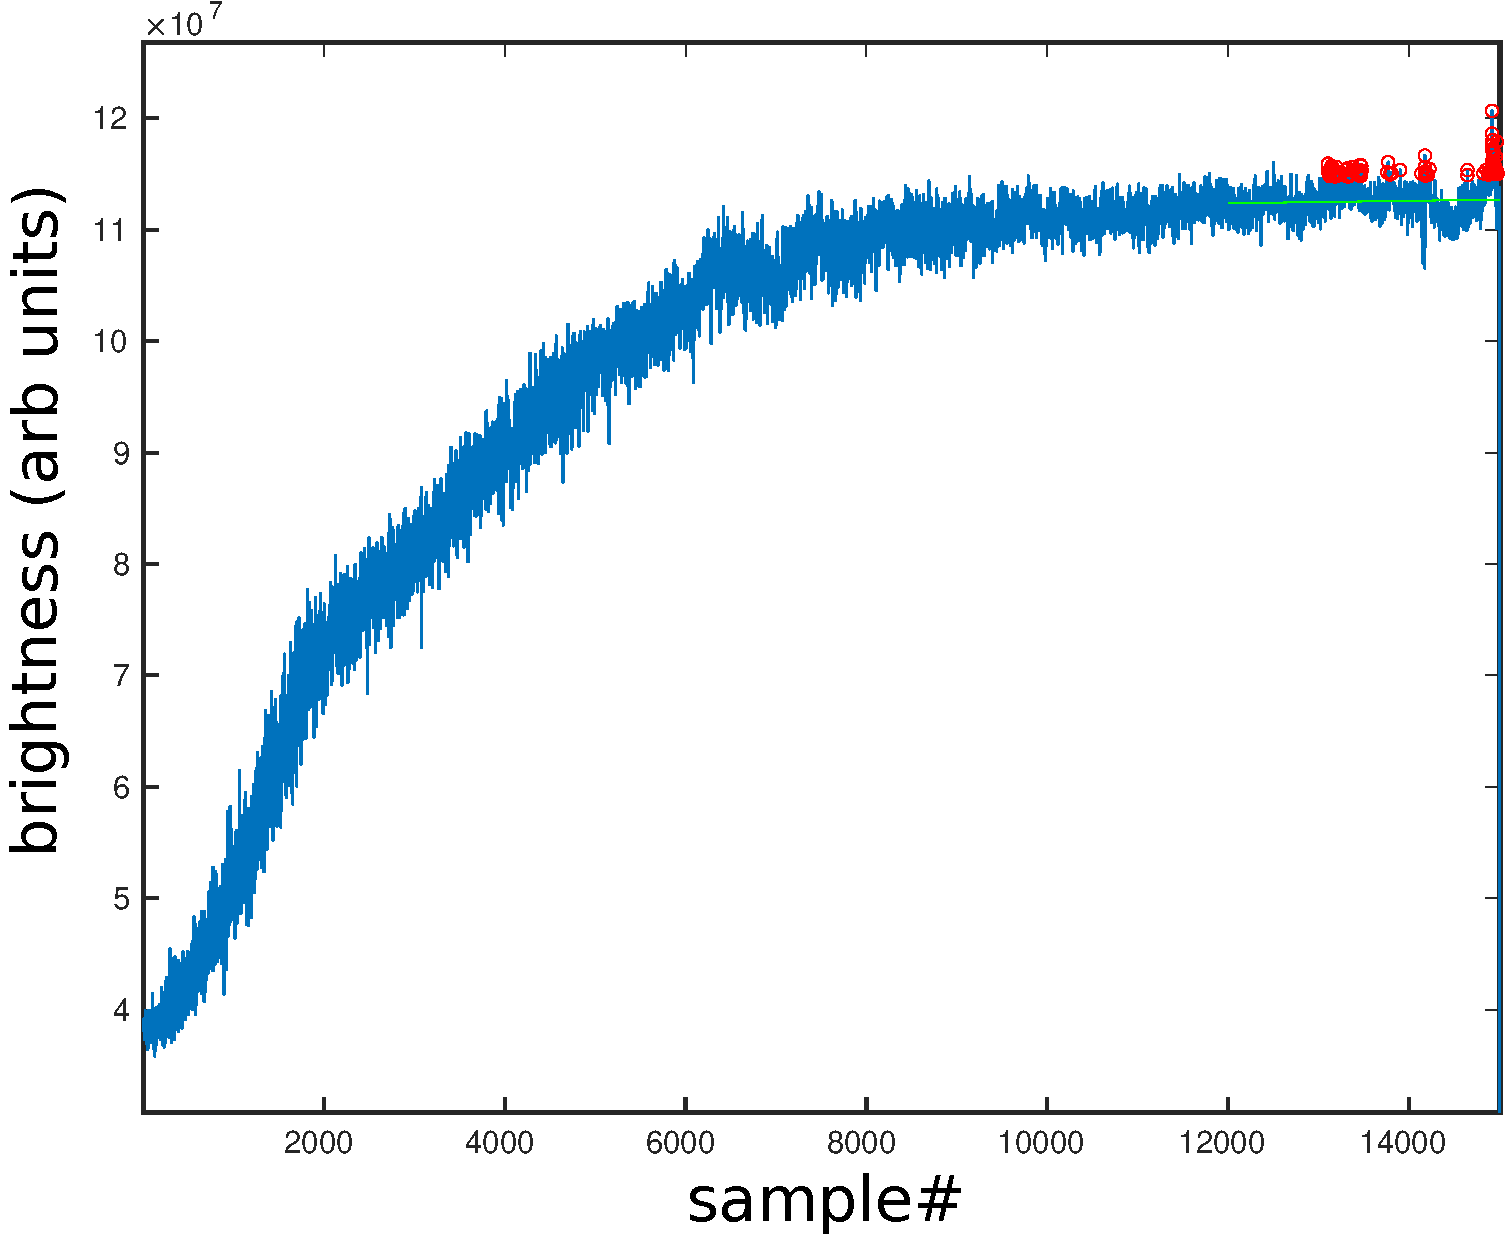
\includegraphics[width=\textwidth]{PSbeads_optimization_run.pdf}
\caption{Example run showing ~3.5x improvement in brightness from naive (no command signal written to the DM).  This was done with PS beads embedded in coverslip sealant; due to the absence of diffusive oxygen, bleaching was almost absent, and this serves as the best calibration to date.}
\end{figure}

\section{Experimental testing}

\subsection{Perliminary testing in slices}

At the beginning of the pandemic, some time testing and validating the system in acute mouse brain slices.  This, unsurpsiingly, is a challenging task; I never did get  calcium transitents, but was able to validate imaging two-color imaging of morphology. Chris Magnus was particuarly helpful in guiding me on the making and maitenance of slices.  

[insert an early image here].  

\subsection{GluSnFR3}

This is so exciting so exciting. 

\section{Conclusions}

\end{document}
